\documentclass[11pt,a4paper]{article}
\usepackage[margin=2.5cm]{geometry}
\usepackage{amsmath,amssymb}
\usepackage{booktabs}
\usepackage{array}
\usepackage{xcolor}
\usepackage{tcolorbox}
\tcbuselibrary{skins,breakable}
\usepackage{enumitem}
\usepackage{hyperref}
\usepackage[numbers,sort&compress]{natbib}
\bibliographystyle{unsrtnat}
\usepackage{tikz}
\usetikzlibrary{arrows.meta,shapes.geometric,positioning,fit,backgrounds}
\hypersetup{colorlinks=true,linkcolor=blue!60!black,urlcolor=blue!60!black}
\setlength{\emergencystretch}{2em}

\definecolor{boxblue}{RGB}{220,235,255}
\definecolor{boxorange}{RGB}{255,240,210}
\definecolor{boxgreen}{RGB}{220,245,220}
\definecolor{boxpurple}{RGB}{240,220,255}
\definecolor{boxred}{RGB}{255,220,220}

\newcommand{\term}[1]{\textbf{#1}}
\newcommand{\lean}[1]{\texttt{#1}}

\title{\textbf{Computational Universality of the Substrate}\\[6pt]
Undecidability, Self-Reference, and Why the Universe Can't Know Itself Completely\\[4pt]
\normalsize\textit{UGP Physics Tutorial Series}
\\[2pt]\small\href{https://doi.org/\TutorialDOI}{doi.org/\TutorialDOI}}
\author{Nova Spivack\\[4pt]
\normalsize
\href{https://novaspivack.com/research}{novaspivack.com/research}\\[2pt]
\small Full monograph (P48):
\href{https://doi.org/10.5281/zenodo.20560550}{doi.org/10.5281/zenodo.20560550}
}
\newcommand{\TutorialDOI}{10.5281/zenodo.20657915}
\date{2026}

\begin{document}
\setcounter{tocdepth}{2}
\maketitle
\tableofcontents
\newpage

\begin{tcolorbox}[colback=blue!6,colframe=blue!40!black,
  title=\textbf{UGP Physics Tutorial Series}]
\textbf{Prerequisites (read first):}
\href{https://doi.org/10.5281/zenodo.20657889}{\emph{The GTE Polynomial: A Step-by-Step Cheat Sheet}}
$\cdot$ \href{https://doi.org/10.5281/zenodo.20657919}{\emph{How the UWCA Works}}
$\cdot$ \href{https://doi.org/10.5281/zenodo.20657895}{\emph{Perfect Self-Containment and MDL}}\\[4pt]
\textbf{Next tutorials:} \href{https://doi.org/10.5281/zenodo.20657910}{\emph{Transputation: The Physics of Measurement}}
$\cdot$ \href{https://doi.org/10.5281/zenodo.20657861}{\emph{The Born Rule as a Theorem}}\\[4pt]
\textbf{See also:} \href{https://doi.org/10.5281/zenodo.20657913}{\emph{From the Arithmetic Substrate to Particle Masses}}
\end{tcolorbox}

\begin{tcolorbox}[colback=boxgreen,colframe=green!50!black,
  title=\textbf{Claim-Strength Taxonomy}]
Throughout this tutorial, results are labeled with a confidence grade:
\begin{itemize}[itemsep=2pt]
  \item \textbf{$\mathbf{A}_{\rm Lean}$ (CatAL)} --- Machine-certified in Lean~4 with zero \texttt{sorry} and zero custom axioms.  Independently verifiable by anyone with Lean installed.
  \item \textbf{A/D (CatAD)} --- Analytically derived with full derivation, computationally confirmed.  Not yet machine-certified.
  \item \textbf{A (CatA)} --- Analytically derived; derivation complete but not independently machine-certified.
  \item \textbf{A/D (conditional)} --- Derived under a named, stated premise; the premise is itself an open problem or a CatB assumption.
  \item \textbf{B (CatB)} --- A stated working hypothesis or structural premise; not yet derived.
\end{itemize}
\end{tcolorbox}

\bigskip
\begin{tcolorbox}[colback=boxpurple,colframe=purple!50!black,title=\textbf{The Central Claim}]
The substrate of the universe is computationally universal — it can, in principle,
simulate any computation whatsoever.  This is not an accident and not a design choice:
it is forced by the requirement that the universe contain its own complete description.
A universe that was \emph{less} than universal could always be described from outside
itself — violating the foundational axiom of self-containment.  But a computationally
universal substrate immediately implies — via Turing's 1936 theorem — that some physical
predictions are formally undecidable.  The universe is, in a precise technical sense,
incomplete about itself.
\end{tcolorbox}

%─────────────────────────────────────────────────────────────────────────────
\section{What Is Computation?}
%─────────────────────────────────────────────────────────────────────────────

\subsection{The mechanical ideal}

A \term{computation} is any process that takes an input and produces an output by
following a fixed sequence of unambiguous rules.  Long division is a computation: given
two numbers, apply a recipe of steps, get a quotient.  Sorting a list is a computation.
Determining whether a number is prime is a computation.

What makes a process a computation — and not just a physical event — is that
\emph{no judgment is needed at any step}: every action is determined by the current
state and the rule.  A computation is fully mechanical.  You could carry it out with
pencil and paper, given enough time.

\subsection{The Turing machine}

In 1936, Alan Turing formalized this intuition into the model now called a
\term{Turing machine}: an infinite paper tape divided into cells, a read/write head
positioned at some cell, and a finite table of rules that says ``if you are in state $q$
and you read symbol $s$, write symbol $s'$, move left or right, and go to state $q'$.''

The tape is the memory.  The state is the current context.  The rule table is the
program.  Given an initial tape (the input), the machine runs until it halts — or
runs forever.

\begin{tcolorbox}[colback=boxblue,colframe=blue!40!black,title=Why Turing machines matter]
Despite their simplicity, Turing machines can compute \emph{everything that any
computer — past, present, or future — can compute}.  Your laptop is, in principle, no
more powerful than a Turing machine: it runs the same problems, just faster.
This equivalence is backed by decades of theoretical work.
\end{tcolorbox}

\subsection{What ``computable'' means}

A function $f$ is \term{computable} if there exists a Turing machine that, given any
valid input, produces the correct output $f(\text{input})$ in finitely many steps.

Examples of computable functions: addition, multiplication, primality testing, sorting,
image compression, chess evaluation.  Every algorithm you have ever heard of computes
a computable function.

\subsection{The Church--Turing thesis}

The \term{Church--Turing thesis} says: every ``reasonable'' model of computation —
abacuses, neural networks, quantum computers, biological brains (in their
information-processing aspects), cellular automata, Python scripts — is equivalent to
a Turing machine in terms of what it can compute.  They may differ in \emph{speed}, but
not in \emph{capability}.

This is not a theorem (it cannot be, since ``reasonable'' is not a mathematical term),
but it has survived every challenge for ninety years.  No one has ever found a
physically realizable process that computes something a Turing machine cannot.

%─────────────────────────────────────────────────────────────────────────────
\section{What Is Computational Universality?}
%─────────────────────────────────────────────────────────────────────────────

\subsection{The key idea}

A system is \term{computationally universal} if it can simulate any Turing machine —
that is, if it can compute any computable function.  A universal system can, in
principle, do anything a computer can do, given enough time and space.

\begin{tcolorbox}[colback=boxorange,colframe=orange!60!black,title=The analogy]
A \textbf{non-universal system} is like a pocket calculator: it can only do arithmetic.
No matter how you configure it, it cannot play chess or sort a list.\\[4pt]
A \textbf{universal system} is like a general-purpose computer: given the right program
(initial state), it can simulate any other computer, including other universal systems.
It can play chess, sort lists, compute primes — anything.
\end{tcolorbox}

\subsection{The surprising simplicity of universal systems}

You might expect that only very complex systems are universal.  This turns out to be
spectacularly wrong.

\term{Rule~110} is a cellular automaton with just 2 possible cell states (0 or 1) and
a neighborhood of 3 cells.  Its update table has 8 rows.  It is, by every measure, one
of the simplest possible dynamical systems.  Yet in 1994, Matthew Cook proved that
Rule~110 is computationally universal: given the right initial pattern on the tape,
it can simulate any Turing machine \cite{Cook2004}.

This is a landmark result.  It says: \emph{extreme simplicity does not preclude
extreme computational power}.  The gap between ``simple rule'' and ``can do anything
computable'' is not bridged by adding complexity; it is bridged by the right kind
of structure.

\subsection{Rule 110's update table}

Rule~110 assigns to each triple $(L, C, R) \in \{0,1\}^3$ a new center-cell value:

\bigskip
\begin{center}
\begin{tabular}{ccc|c}
\toprule
$L$ & $C$ & $R$ & New $C$ \\
\midrule
0 & 0 & 0 & 0 \\
0 & 0 & 1 & 1 \\
0 & 1 & 0 & 1 \\
0 & 1 & 1 & 1 \\
1 & 0 & 0 & 0 \\
1 & 0 & 1 & 1 \\
1 & 1 & 0 & 1 \\
1 & 1 & 1 & 0 \\
\bottomrule
\end{tabular}
\end{center}
\bigskip

Reading the output column bottom-to-top gives the binary number $01101110_2 = 110_{10}$
— hence ``Rule~110.'' The rule can simulate any algorithm because it can support stable
propagating structures (``gliders'') and collision rules between them that implement
Boolean logic gates — from which anything computable can be built.

%─────────────────────────────────────────────────────────────────────────────
\section{The Substrate's Universality: The Two-Path Argument}
%─────────────────────────────────────────────────────────────────────────────

\begin{tcolorbox}[colback=boxgreen,colframe=green!50!black,title=The GTE polynomial]
\[
  p(L,\,C,\,R) \;=\; C + R - CR - LCR \pmod{7}
\]
The GTE framework~\cite{SpivackGTECompleteFramework} is built on this single degree-3 polynomial over the 7-element
field~GF(7).  When restricted to binary inputs $\{0,1\}$, it computes Rule~110 exactly.
\end{tcolorbox}

\smallskip
\noindent\textbf{Two-level note.}
The polynomial $p$ is GTE's Level~1 \emph{algebraic certificate} — it certifies which
structures the universe must contain.
The physical universe is the Level~2 $\Phi_{\mathrm{MDL}}$ field
($\mathcal{L} = \tfrac{1}{2}(\partial_\mu\Phi)^2
- \tfrac{m^2}{49}(1{-}\cos 7\Phi) + \mathcal{L}_{\rm gauge}$),
whose BPS kink solitons are the elementary particles.
The universality results in this tutorial hold at the algebraic layer (Level~1);
see the \emph{The $\Phi_{\mathrm{MDL}}$ Field} and \emph{Particles as Kinks}
tutorials for the Level~2 physical derivation.

\smallskip
The GTE substrate inherits Rule~110's universality via two completely independent
proofs~\cite{SpivackCompUniversality}.  Both paths are machine-certified in Lean~4 with zero sorry and zero custom
axioms.

\subsection{Path~1: From above — the UWCA substrate}

The \term{UWCA} (Universal Wireworld Cellular Automaton) is the native computation
engine built into the UGP arithmetic substrate.  Its architecture uses four passes
per round (P1--P4) to update each cell: detect active neighborhoods, compute flags,
aggregate results, commit.

The key theorem proves that one full UWCA round implements exactly one step of
Rule~110:
\[
  \lean{uwca\_sweep\_implements\_rule110} \quad (\text{CatAL, zero sorry})
\]
Formally: for any tape in the binary sector, after one UWCA sweep, cell $i$ holds
the value $\mathrm{rule110Output}(C_{i-1}, C_i, C_{i+1})$.  Since Rule~110 is
Turing-universal, the UWCA — and the substrate it runs on — is Turing-universal.

\subsection{Path~2: From below — the orbit parity shadow}

The GTE orbit is a specific sequence of integer triples generated by the map $T$
starting from the Lepton Seed $(1, 73, 823)$ at ridge level $n=10$.
When every coordinate of every orbit triple is reduced modulo 2 (``the parity shadow''),
the resulting binary triples fill in 7 of the 8 rows of a binary truth table.
Each binary triple is obtained by reading three consecutive ring positions
$(g_{i-1},\,g_i,\,g_{i+1})$ from an orbit state modulo~2 as CA inputs $(L,C,R)$
and recording the next-step center value $g_i'$ modulo~2 as the Rule~110 output;
the orbit's arithmetic forces these reduced input--output pairs to trace exactly the
Rule~110 entries.
The 8th row is fixed by the vacuum-transparency condition (the all-zeros state must be
a fixed point).

The theorem \lean{cup1\_orbit\_uniquely\_selects\_rule110} (CatAL) proves that the
unique multilinear polynomial consistent with all 8 rows is the Rule~110 truth table —
not approximately, but exactly, as a forced algebraic consequence of the orbit's
arithmetic.

The GTE polynomial's binary restriction is Rule~110 not by design but because
\emph{the orbit's own arithmetic forces it}.

\subsection{Two paths, one universal substrate}

\begin{tcolorbox}[colback=boxblue,colframe=blue!40!black,
  title=The two universality certificates]
\begin{itemize}
\item \textbf{Path~1 (UWCA, from above):} The UWCA sweep implements Rule~110 cell by cell.\\
  \lean{uwca\_sweep\_implements\_rule110} (CatAL, zero sorry).
\item \textbf{Path~2 (Orbit parity, from below):} The GTE orbit's parity shadow forces
  the binary restriction of $p$ to be Rule~110 exactly.\\
  \lean{cup1\_orbit\_uniquely\_selects\_rule110} (CatAL, zero sorry).
\item \textbf{Algebraic route (independent):} $p(L,1,R) = 1 - LR = \mathrm{NAND}(L,R)$
  (mod 7), and NAND is functionally complete (Sheffer 1913).\\
  \lean{rule110\_turing\_universal\_algebraic} (CatAL, zero sorry).
\end{itemize}
Three independent proofs from three independent mathematical directions all certify
the same conclusion: the GTE substrate is computationally universal.
\end{tcolorbox}

%─────────────────────────────────────────────────────────────────────────────
\section{Why Perfect Self-Containment Requires Universality}
\label{sec:psc-forces-universality}
%─────────────────────────────────────────────────────────────────────────────

This is the key section.  Everything else in this tutorial follows from the argument
here.  Read it slowly.

\subsection{The foundational axiom: Reflexive Closure}

The GTE framework is built on a foundational condition called
\term{Perfect Self-Containment} (PSC).  PSC formalizes the idea that the universe has
no ``outside'': no external observer selects its laws, no external mechanism runs its
dynamics, no external description completes its specification.

The universe is a closed system, all the way down.

PSC is formalized through five axioms.  The one relevant here is called
\term{Reflexive Closure} (RC):

\begin{tcolorbox}[colback=boxblue,colframe=blue!40!black,title=Reflexive Closure (RC)]
The universe must contain its own complete description.  Formally: the universe $U$
is its own law $L(U)$: 
\[
  S = L(S)
\]
The description, the law, and the substrate that executes both are all the same object.
No part of the specification lives outside the system.
\end{tcolorbox}

\subsection{The multi-step argument}

Now we build the logical chain, step by step.

\medskip
\textbf{Step~1: A complete description of a dynamical universe is an executable program.}

A ``complete description'' is not a picture or a static list of facts.  A description of
a dynamical system that is complete must include the rules governing the system's
evolution.  To be a complete description, it must be able to answer: ``what happens
next?''  That makes it executable.  A complete description is a program.

\medskip
\textbf{Step~2: What does ``executable from inside'' mean?}

Reflexive Closure says the description lives inside the universe.  The substrate that
runs the dynamics is the same substrate that contains the description.  For the
description to be executable — to be able to simulate the universe — the substrate
must be able to run it.

\medskip
\textbf{Step~3: A sub-universal substrate always has a complete external description.}

Suppose the substrate could only run a restricted class of computations — say, only
arithmetic, or only sorting, or only cellular automata up to some fixed complexity bound.
Such a substrate is \term{sub-universal}: there exist programs it cannot run.

But a sub-universal substrate is, by definition, simpler than a Turing machine.
And anything simpler than a Turing machine can be exactly simulated by a Turing machine.
A Turing machine can represent the sub-universal system's state as a data structure and
faithfully evolve it step by step.  In other words: a sub-universal substrate has a
complete external description — one that could be written down and run by a system
outside it.

\medskip
\textbf{Step~4: PSC forbids any complete external description.}

RC says: $S = L(S)$.  The universe is its own law, not a law that some other system
could also express.  If the universe had a complete external description, then something
outside the universe could fully specify it.  But PSC says there is nothing outside.

\begin{tcolorbox}[colback=boxred,colframe=red!50!black,title=The contradiction]
If the substrate is sub-universal, it has a complete external description (Step~3).\\
But PSC forbids any complete external description (Step~4).\\
\textbf{Therefore the substrate cannot be sub-universal.}
\end{tcolorbox}

\textbf{Step~5: The only escape is universality.}

The only substrates without a complete external description are those that can simulate
any Turing machine — universal substrates.  A Turing-universal system can represent
any computable description of itself, but no computable description is complete (we will
see why in Section~\ref{sec:pit}).  Universality is the one-and-only structure that
satisfies RC without allowing an external description.

\begin{tcolorbox}[colback=boxgreen,colframe=green!50!black,
  title=The PSC-Universality Theorem]
A PSC-consistent universe must have a computationally universal substrate.\\
Sub-universality implies external describability, which contradicts RC.\\
Therefore: $\text{PSC} \;\Rightarrow\; \text{computational universality}$.
\end{tcolorbox}

\subsection{The elevator analogy}

Here is an intuitive way to hold the argument:

Imagine a universe inside an elevator with no buttons and no shaft visible from
inside.  If the elevator were a simple mechanism — say, it only goes up and down
— an engineer standing outside could fully describe its operation: ``it has two
states, up-button pressed and down-button pressed, and the transition function is...''

The engineer's description is external and complete.  The elevator has no inside
knowledge of the engineer, but the engineer has complete knowledge of the elevator.

PSC says: our universe is not an elevator.  There is no engineer outside.  No external
description is complete.  For this to be true, the universe must be genuinely
complex enough that no external system can capture it in a finite description.
The minimum requirement for this is computational universality.

%─────────────────────────────────────────────────────────────────────────────
\section{The Undecidability Consequence: The Physical Incompleteness Theorem}
\label{sec:pit}
%─────────────────────────────────────────────────────────────────────────────

\subsection{Turing's halting theorem}

In 1936, Turing proved that no algorithm can decide, for an arbitrary program and input,
whether the program eventually halts or runs forever.  This is the
\term{halting problem}, and it is \emph{undecidable}: there is no Turing machine $H$
such that $H(P, x) = 1$ if program $P$ halts on input $x$, and $H(P, x) = 0$ if it
does not.

The proof is a \term{diagonal argument}: assume $H$ exists, construct a program $D$
that calls $H$ on itself and does the opposite of what $H$ predicts.  $D$ halts if
and only if $H$ says it doesn't, which is a contradiction.  So $H$ cannot exist.

\begin{tcolorbox}[colback=boxblue,colframe=blue!40!black,title=Key insight]
The halting problem is not merely \emph{hard} — it is formally and permanently
\emph{impossible} to solve algorithmically.  No increase in computing speed, memory,
or algorithmic cleverness can change this.
\end{tcolorbox}

\subsection{Applying Turing's theorem to physics}

Once the physical substrate is computationally universal, Turing's theorem immediately
applies to it.  This is the content of the \term{Physical Incompleteness Theorem} (PIT).

The PIT follows from three premises:
\begin{enumerate}
\item \textbf{(PhysUCT)} The physical substrate is Turing-universal\\
  (certified: \lean{phimdl\_turing\_universal}, CatAL, zero sorry).
\item \textbf{(PSC)} The universe satisfies Reflexive Closure: the substrate must
  encode its own complete description (Section~\ref{sec:psc-forces-universality}).
\item \textbf{(ASR)} The universe can form statements about its own computational
  behavior — it contains an arithmetic self-reference structure.  This follows from
  (1) + (2) by the standard Gödel self-reference construction.
\end{enumerate}

From these three premises:

\begin{tcolorbox}[colback=boxorange,colframe=orange!60!black,
  title={PIT Form~A: Computational Undecidability (CatAL)}]
The predicate ``physical process $X$ eventually reaches a definite outcome $w$'' is
not computably decidable.  No algorithm running on the physical substrate can predict
all measurement outcomes on the self-referential diagonal fragment.\\[4pt]
Machine-certified: \lean{asr\_rt\_not\_computable} (CatAL, NEMS Paper~11,
zero sorry, zero custom axioms; via Mathlib \texttt{halting\_problem}).
\end{tcolorbox}

\begin{tcolorbox}[colback=boxorange,colframe=orange!60!black,
  title={PIT Form~B: No Final Self-Theory (CatAL)}]
No PSC-consistent theory can contain a complete account of its own physics.
The universe cannot write its own complete user manual.\\[4pt]
Machine-certified: \lean{no\_final\_self\_theory} (CatAL, zero sorry;
NEMS Paper~51).
\end{tcolorbox}

\subsection{What does this mean physically?}

The vast majority of physics is unaffected.  Particle masses, coupling constants,
cosmological parameters, all Standard Model predictions — these are derivable from the
GTE structure with no undecidability.

What is undecidable is the specific outcome of any individual quantum measurement event
on the \emph{self-referential diagonal fragment}: the specific decay time of a
radioactive atom, the specific outcome of a spin-up-or-down measurement.

These are precisely the events that standard quantum mechanics also declares
unpredictable.  What GTE adds is a \emph{derivation} of why: they are unpredictable
not by postulate, not by convention, but because they are formally equivalent to the
halting problem applied to the universe's own description.

\begin{tcolorbox}[colback=boxblue,colframe=blue!40!black,title=PIT vs.\ Gödel and Turing]
\textbf{Gödel incompleteness (1931):} Mathematical systems cannot prove all true
  statements about themselves.  The gap is in \emph{proof}.\\[4pt]
\textbf{Turing halting problem (1936):} No algorithm can decide all questions
  about computations.  The gap is in \emph{computation}.\\[4pt]
\textbf{PIT (GTE):} No physical substrate can algorithmically predict all of its
  own measurement outcomes.  The gap is in \emph{physics}: it is about
  measurement, not abstract proof or abstract computation.
\end{tcolorbox}

\subsection{Feature, not bug}

Physical incompleteness is not a flaw in GTE.  It is the necessary consequence of
PSC closure.

A universe that could fully predict all of its own measurement outcomes would need an
internal procedure that decides all self-referential questions about its substrate.
But no such procedure exists (PIT).  A universe that \emph{were} fully
self-predictable would violate PSC.

Stated another way: the universe's inability to fully predict itself is
precisely what allows it to be a closed system with no outside.
The incompleteness is built in; it is the price of having no external observer.

%─────────────────────────────────────────────────────────────────────────────
\section{The Degree $\mathbf{0}'$ Classification}
%─────────────────────────────────────────────────────────────────────────────

The PIT does not merely say ``some physical predictions are undecidable.''
It pins down \emph{precisely how undecidable} they are, using the rigorous concept of
\term{Turing degrees}.

\subsection{The Turing degree hierarchy}

Turing degrees measure the computational complexity of a problem by asking:
``Which problems can a Turing machine solve if given a solution to this one as a free
oracle?''

\begin{itemize}
\item \textbf{Degree $\mathbf{0}$} — Computable problems: standard Turing machines solve
  them without any oracle.  Addition, primality testing, sorting.

\item \textbf{Degree $\mathbf{0}'$} — The halting degree: problems solvable with a halting
  oracle (``does this program halt?''), but not without.  The halting problem itself
  has degree $\mathbf{0}'$.

\item \textbf{Degree $\mathbf{0}''$} — Problems requiring two jumps: a halting oracle
  plus a second oracle for the halting problem relativized to the first oracle.  And so on.
\end{itemize}

Higher degrees are progressively harder.  Degree $\mathbf{0}$ is what Turing machines
compute unaided.  Every higher degree requires at least one non-computable ``jump.''

\subsection{The branch selector is exactly $\mathbf{0}'$}

GTE's transputation operator — the internal adjudicator that selects which quantum
branch is realized at each measurement event — has been classified:

\begin{tcolorbox}[colback=boxpurple,colframe=purple!50!black,
  title={The Turing-Degree Classification Theorem (CatAL)}]
The decision-theoretic restriction of the branch-selection function to the
self-referential diagonal has Turing degree \emph{exactly} $\mathbf{0}'$ — neither
more nor less than the halting degree.\\[4pt]
Specifically: record-truth on the diagonal is $\Sigma^0_1$-complete via a
many-one reduction \lean{halting\_manyOne\_reducible\_to\_RT} (CatAL).
The adjudicator is limit-computable by a stage sequence with a bounded mind-change
count ($\leq 8$ for single-kink events), but admits no computable convergence modulus
\lean{no\_computable\_convergence\_modulus} (CatAL, nems-lean).
\end{tcolorbox}

\subsection{Why exactly $\mathbf{0}'$ and not more?}

Two bounds fix the degree from both sides:

\textbf{Lower bound (not degree $\mathbf{0}$):} If the branch selector were computable,
the PIT would be violated.  There would exist an algorithm that decides all
measurement outcomes on the diagonal fragment, contradicting \lean{asr\_rt\_not\_computable}.
So the degree is strictly above $\mathbf{0}$.

\textbf{Upper bound (not degree $\mathbf{0}''$ or higher):} The PSC-admissible
candidate set is Turing-enumerable — the universe selects from a well-structured,
computable list of options.  A single non-computable selection event of this type
does not provide a general oracle for higher-order questions.
Lean-certified: \lean{transputation\_not\_reducible\_to\_total\_effective\_computation}
(CatAL, zero sorry, transputation-lean).

Together: exactly one Turing jump above the computable.  Exactly $\mathbf{0}'$.

\subsection{The physical interpretation}

\begin{tcolorbox}[colback=boxblue,colframe=blue!40!black,title=Plain English]
The universe, at the level of individual quantum measurement outcomes, performs
operations that are exactly as hard as the halting problem.  Not harder — it is not
doing anything that would require solving an oracle Turing machine.  Not easier — it is
not doing something a Turing machine could do.  Exactly the first level of
non-computability.

This is why quantum randomness feels irreducible: it is not just practically
unpredictable but formally, provably, and exactly as unpredictable as deciding
whether an arbitrary program halts.
\end{tcolorbox}

For more on what performs these degree-$\mathbf{0}'$ adjudications physically, see the
Transputation Tutorial.

%─────────────────────────────────────────────────────────────────────────────
\section{The Entropy Argument: Why Exact Universality at Minimum Cost}
%─────────────────────────────────────────────────────────────────────────────

\subsection{Universality is not a spectrum}

A common intuition: ``maybe the universe is only somewhat universal, or universal
in some restricted sense.''  There is no such thing.  Universality is binary: a system
either can simulate any Turing machine, or it cannot.  The GTE substrate is certified
universal.

But a sharper question remains: \emph{why exactly this universal system, and not
another?}

\subsection{MDL selects the minimal universal system}

Among all possible cellular automaton rules, some are not universal (they cannot
simulate arbitrary computations) and some are.  Among universal rules, they differ in
complexity: some require more bits to specify than others.

The \term{Minimum Description Length} (MDL) principle — the third axiom of UGP, itself
derived from the Presentation Invariance axiom of PSC — selects the shortest complete
description.  Applied to the space of all $k=7$, $r=1$ cellular automaton rules,
MDL asks: which valid rule has the shortest description?

The answer is machine-certified:

\begin{tcolorbox}[colback=boxgreen,colframe=green!50!black,title=The 19-bit result (CatAMDL)]
The GTE polynomial $p(L,C,R) = C + R - CR - LCR$ (mod~7) has a description length of
exactly \textbf{19 bits}:
\begin{center}
\begin{tabular}{ll}
\toprule
Component & Bits \\
\midrule
Binary restriction (Rule~110 truth table) & 8 bits \\
Prime modulus ($\lceil\log_2 7 \rceil = 3$) & 3 bits \\
Monomial selector (which of 8 basis monomials are nonzero) & 5 bits \\
Chirality (left--right orientation) & 1 bit \\
Sign of the $-1$ coefficients & 2 bits \\
\midrule
Total & 19 bits \\
\bottomrule
\end{tabular}
\end{center}
A naive lookup table for the same rule requires $343 \times \log_2 7 \approx 963$~bits
— about 50 times larger.  No shorter valid description exists (MDL Uniqueness Theorem,
CatAMDL; machine-certified in Lean~4, zero sorry).
\end{tcolorbox}

\subsection{The remarkable coincidence}

Why is this remarkable?

Among all valid rules (those passing the physics-admissibility constraints of PSC),
$p$ is the shortest.  But it is also computationally universal — its binary restriction
is Rule~110.

These two properties appear unrelated.  Minimality is about description length.
Universality is about what computations the rule can perform.  Yet both properties are
achieved simultaneously by the same object.

The explanation is structural, not coincidental: MDL selects the rule that is
minimally complex while still passing all PSC constraints.  PSC's Reflexive Closure
requires universality.  Therefore the MDL-minimal PSC-consistent rule must be
universal.  The minimum-cost PSC-consistent description lands exactly at the
universality threshold — which is Rule~110.

\begin{tcolorbox}[colback=boxblue,colframe=blue!40!black,title=The key insight]
The universe achieves computational universality at the minimum possible descriptive
cost.  It is not over-engineered: 19 bits is the price of admission for a
self-consistent universe with no external description.  Any rule with fewer bits would
be sub-universal and would violate PSC.  Any rule with more bits would be redundant.
The MDL functional selects exactly one rule — and it happens to be the one that
produces the Standard Model.
\end{tcolorbox}

%─────────────────────────────────────────────────────────────────────────────
\section{The Full Chain of Implications}
%─────────────────────────────────────────────────────────────────────────────

\begin{tcolorbox}[colback=boxpurple,colframe=purple!50!black,
  title=The Complete Logical Chain]
\begin{enumerate}
\item \textbf{PSC}: the universe is self-contained — no external description, no
  external dynamics, no external law-selector.
\item \textbf{$\Rightarrow$ Sub-universality is ruled out}: a sub-universal substrate
  can always be described by a strictly larger system — giving it a complete external
  description, violating PSC.
\item \textbf{$\Rightarrow$ The substrate must be computationally universal}: Rule~110
  is the minimal universal rule; the GTE substrate achieves universality from two
  independent directions (UWCA path, orbit parity path).
\item \textbf{$\Rightarrow$ Turing's theorem applies}: a universal physical substrate
  means some physical questions are formally undecidable.
\item \textbf{$\Rightarrow$ Physical Incompleteness Theorem}: no total-effective
  algorithm can predict all quantum measurement outcomes on the self-referential fragment.\\
  \lean{asr\_rt\_not\_computable} (CatAL, zero sorry).
\item \textbf{$\Rightarrow$ Branch selector must be non-computable}: physical selection
  still occurs (every quantum event has a definite outcome), so PSC forces an internal
  non-computable adjudicator — transputation.\\
  \lean{PSC\_and\_choice\_force\_PT} (CatAL, zero sorry).
\item \textbf{$\Rightarrow$ Turing degree exactly $\mathbf{0}'$}: the adjudicator is
  limit-computable (one halting jump above computable) but not computably convergent.\\
  \lean{halting\_manyOne\_reducible\_to\_RT} (CatAL).
\item \textbf{$\Rightarrow$ Born rule is a theorem}: PSC forces probability assignments
  to be non-contextual and POVM-additive; Gleason's theorem then uniquely selects the
  Born-rule density-operator form.\\
  \lean{busch\_gleason\_unique} (CatAL, zero sorry).
\item \textbf{$\Rightarrow$ MDL selects the 19-bit polynomial as the minimal-cost
  universal rule}: no shorter valid rule exists; any shorter rule is sub-universal
  and violates PSC.
\item \textbf{$\Rightarrow$ Physical predictions are derivable from the polynomial's
  structure}: particle masses, gauge groups, cosmological observables — all from $p$.
\end{enumerate}
\end{tcolorbox}

Below is the same chain presented as a flowchart.

\bigskip

\begin{center}
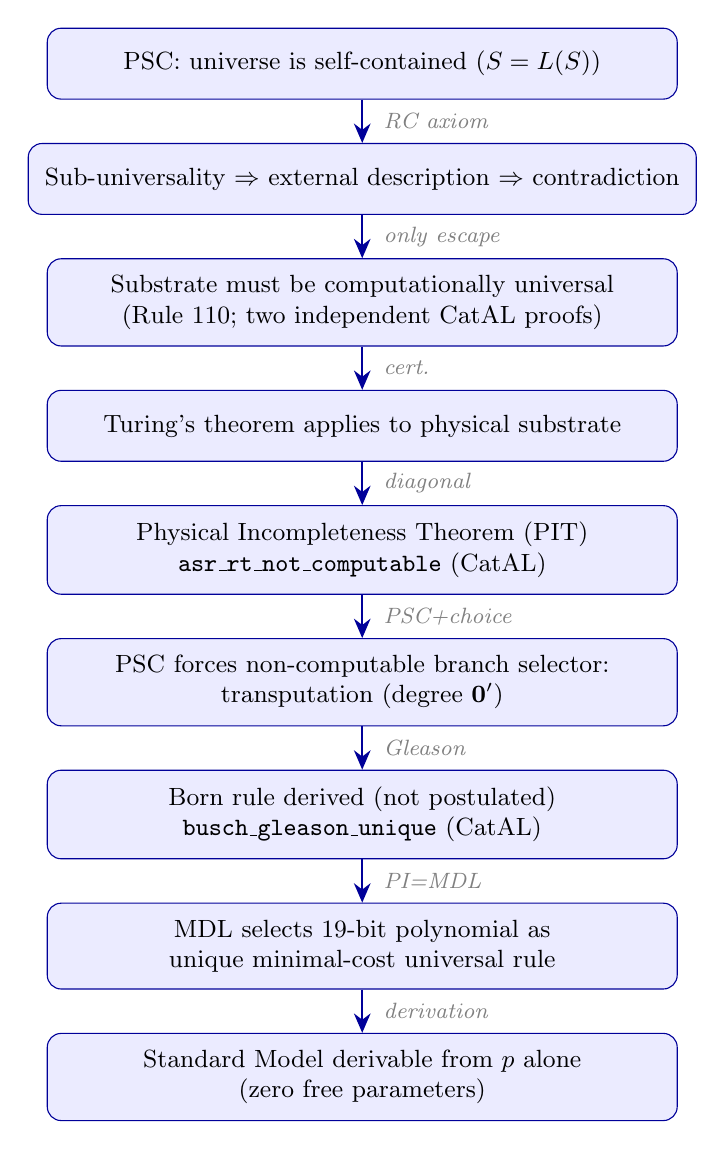
\begin{tikzpicture}[
  box/.style={draw=blue!60!black, fill=blue!8, rounded corners=5pt,
              align=center, font=\small, inner sep=6pt, minimum width=8cm,
              minimum height=0.9cm},
  arr/.style={-{Stealth[length=7pt,width=6pt]}, thick, blue!60!black},
  ann/.style={font=\footnotesize\itshape, text=gray, midway, right, xshift=4pt},
]
\node[box] (psc) {PSC: universe is self-contained ($S = L(S)$)};
\node[box, below=0.55cm of psc] (noext) {Sub-universality~$\Rightarrow$~external description~$\Rightarrow$~contradiction};
\node[box, below=0.55cm of noext] (univ) {Substrate must be computationally universal\\
  (Rule~110; two independent CatAL proofs)};
\node[box, below=0.55cm of univ] (turing) {Turing's theorem applies to physical substrate};
\node[box, below=0.55cm of turing] (pit) {Physical Incompleteness Theorem (PIT)\\
  \small\lean{asr\_rt\_not\_computable} (CatAL)};
\node[box, below=0.55cm of pit] (transp) {PSC forces non-computable branch selector:\\
  transputation~(degree $\mathbf{0}'$)};
\node[box, below=0.55cm of transp] (born) {Born rule derived (not postulated)\\
  \small\lean{busch\_gleason\_unique} (CatAL)};
\node[box, below=0.55cm of born] (mdl) {MDL selects 19-bit polynomial as\\
  unique minimal-cost universal rule};
\node[box, below=0.55cm of mdl] (sm) {Standard Model derivable from $p$ alone\\
  (zero free parameters)};

\draw[arr] (psc) -- (noext) node[ann] {RC axiom};
\draw[arr] (noext) -- (univ) node[ann] {only escape};
\draw[arr] (univ) -- (turing) node[ann] {cert.};
\draw[arr] (turing) -- (pit) node[ann] {diagonal};
\draw[arr] (pit) -- (transp) node[ann] {PSC+choice};
\draw[arr] (transp) -- (born) node[ann] {Gleason};
\draw[arr] (born) -- (mdl) node[ann] {PI=MDL};
\draw[arr] (mdl) -- (sm) node[ann] {derivation};
\end{tikzpicture}
\end{center}

%─────────────────────────────────────────────────────────────────────────────
\section{Why This Is Remarkable}
%─────────────────────────────────────────────────────────────────────────────

\subsection{Most theories assume; GTE derives}

Standard physics takes the laws of nature as given.  They are measured, tabulated,
and then used to make predictions.  The question ``why these laws?'' is left outside
the theory's scope.

PSC does not allow this.  The moment you require the universe to have no external
description, you have imposed a constraint on what the universe can be.  The laws
must emerge from the requirement that the universe be self-consistent and self-contained.

Computational universality is one of the deepest consequences of this requirement.
It is not a separate postulate.  It is not an observation about our universe that
happens to be true.  It is \emph{forced} by the logic of self-containment.

\subsection{The double derivation}

The same 19-bit polynomial that produces the Standard Model particle masses also
produces Rule~110 universality.  These look like two completely different facts about
nature — one quantitative (why is the electron mass what it is?) and one structural
(why is the universe computationally universal?).

In GTE they share a single cause: the polynomial is the unique minimal self-consistent
law.  Universality and physics are not two different things.  They are two aspects
of the same object, seen from different angles.

\subsection{The measurement problem dissolves}

The measurement problem in quantum mechanics asks: how does a definite classical
outcome emerge from a superposition of quantum states?  Standard quantum mechanics
does not answer this — it either ignores the problem (Copenhagen), multiplies it
(many-worlds), or adds extra dynamics (GRW, Penrose).

GTE's answer: the universe performs degree-$\mathbf{0}'$ adjudications at measurement
events via transputation.  These are not algorithmic — they cannot be — because the
PIT forbids it.  But they are determinate and law-governed: every quantum event has
a specific, non-random-in-principle outcome selected by the PSC-forced transputation
operator.

The irreducible randomness of quantum mechanics is not a primitive mystery.  It is a
theorem: formally equivalent to the halting problem, no more mysterious and no less real.

\subsection{The universe that cannot know itself}

The title of this tutorial is a theorem.  The universe contains self-referential
structures (it is computationally universal, and RC requires it to encode its own
description).  By the diagonal argument, any such system encounters statements about
itself that it cannot decide from within.

This is not a limitation that better physics could remove.  It is permanent, formal,
and exactly quantified.  The universe is as incomplete about itself as any
sufficiently powerful formal system — and for exactly the same mathematical reason.

%─────────────────────────────────────────────────────────────────────────────
\section*{Summary}
%─────────────────────────────────────────────────────────────────────────────

\begin{tcolorbox}[colback=boxblue,colframe=blue!40!black,title=What we have shown]
\begin{enumerate}
\item Computation is any mechanical, rule-governed process.  A computationally
  universal system can simulate any such process.
\item Rule~110 is the simplest known computationally universal system.
\item The GTE substrate achieves universality from three independent directions
  (UWCA, orbit parity shadow, algebraic NAND), all machine-certified.
\item Perfect Self-Containment (PSC) requires universality: a sub-universal substrate
  has a complete external description, contradicting the Reflexive Closure axiom.
\item Once the substrate is universal, Turing's theorem forces the Physical
  Incompleteness Theorem: some physical predictions (individual quantum outcomes)
  are formally undecidable.
\item The degree of undecidability is exactly $\mathbf{0}'$ — neither more (no
  hypercomputation) nor less (not computable) — certified by Lean.
\item MDL selects the unique minimal-cost universal rule: 19 bits, producing the
  Standard Model with zero free parameters.
\item Quantum randomness is a theorem, not a postulate: the unavoidable consequence
  of a self-contained computationally universal substrate.
\end{enumerate}
\end{tcolorbox}

%─────────────────────────────────────────────────────────────────────────────
\section*{Further Reading}
%─────────────────────────────────────────────────────────────────────────────

\begin{tcolorbox}[colback=orange!8,colframe=orange!50!black,
  title=\textbf{Primary Sources}]
All papers are open-access on Zenodo and at
\href{https://novaspivack.com/research}{novaspivack.com/research}:
\begin{itemize}
\item \textbf{P48 --- The Complete GTE Framework} (main synthesis monograph):\\
  \href{https://doi.org/10.5281/zenodo.20560550}{doi.org/10.5281/zenodo.20560550}\\
  See especially: Ch.~5 (Binary Universality), Ch.~10 (Measurement and PIT),
  §Physical Incompleteness, §Transputation and Degree $\mathbf{0}'$.

\item \textbf{P28 --- Computational Universality and the Standard Model}\\
  (Rule~110, $\mathbb{Z}_5$ rings, and mod-7 structure in UGP):\\
  \href{https://doi.org/10.5281/zenodo.20259513}{doi.org/10.5281/zenodo.20259513}

\item \textbf{NEMS Paper~11 --- Physical Incompleteness}:\\
  \href{https://doi.org/10.5281/zenodo.19429735}{doi.org/10.5281/zenodo.19429735}\\
  Contains the formal proof of \lean{asr\_rt\_not\_computable}.

\item \textbf{NEMS Paper~05 --- Two-Layer PSC Theorem}:\\
  \href{https://doi.org/10.5281/zenodo.19429721}{doi.org/10.5281/zenodo.19429721}\\
  The theorem that PSC forces $\mathrm{SU}(3)\times\mathrm{SU}(2)\times\mathrm{U}(1)$
  and $N_{\rm gen}=3$.
\end{itemize}
Lean~4 machine proofs (zero sorry, zero custom axioms):\\
\href{https://github.com/novaspivack/ugp-lean}{github.com/novaspivack/ugp-lean}
\end{tcolorbox}

\begin{thebibliography}{9}

\bibitem{Cook2004}
Cook, M.\ (2004).
\newblock Universality in elementary cellular automata.
\newblock \textit{Complex Systems}, 15(1), 1--40.

\bibitem{Turing1936}
Turing, A.\ M.\ (1936).
\newblock On computable numbers, with an application to the Entscheidungsproblem.
\newblock \textit{Proceedings of the London Mathematical Society}, s2-42(1), 230--265.

\bibitem{Sheffer1913}
Sheffer, H.\ M.\ (1913).
\newblock A set of five independent postulates for Boolean algebras, with
  application to logical constants.
\newblock \textit{Transactions of the American Mathematical Society},
  14(4), 481--488.

\bibitem{Godel1931}
Gödel, K.\ (1931).
\newblock Über formal unentscheidbare Sätze der Principia Mathematica und
  verwandter Systeme~I.
\newblock \textit{Monatshefte für Mathematik und Physik}, 38, 173--198.

\end{thebibliography}

\bibliography{../../papers/bib/Spivack_Papers_Bibliography}
\end{document}
